\documentclass[UKenglish]{book}
\newcommand\hmmax{0}
\newcommand\bmmax{0}

\counterwithout{footnote}{chapter}
\usepackage{Setup/style}
\DeclareMathAlphabet{\mathcal}{OMS}{cmsy}{m}{n}
\raggedbottom %%reduces the gaps between the paragraphs
\usepackage{jheppub}

\title{Bayesian neural network estimation of next-to-leading-order cross sections}
%\subtitle{My subtitle}
\subsubtitle{by}
\author{René Alexander Ask}
\thesistext{THESIS}
\thesistextt{for the degree of}
\thesistexttt{MASTER OF SCIENCE}


\bibliographystyle{JHEP}
%\addbibresource{bibliography.bib}
%\DeclareUnicodeCharacter{2212}{-}
%\DeclareUnicodeCharacter{03B1}{-}

\begin{document}
\duoforside[dept={Department of Physics},
  program={Master's Program Name},
  long]
%%%%%%%%%%%%%%%%%%%%%%%%%%%%%%%%%%%%%%%%%%%

\frontmatter{}
\chapter*{Abstract} 
Near the kinematical production threshold scattering cross sections gain large logarithmic corrections. This is due to the fact that close to the threshold the radiation of gauge bosons is restricted to be soft. This leads to an imbalance in the cancelling between real and virtual contributions at higher order, leading to large logarithmic contributions. In order to make reliable predictions such contributions must be resummed. In this thesis we make use of an object called a Wilson line to describe the soft radiation. Wilson lines are path-ordered exponentials of the gauge fields. They contain all the kinematical and dynamical information from the gauge sector and are central in taking a geometrical viewpoint of quantum field theory, and in particular quantum chromodynamics. We mainly consider semi-infinite Wilson lines on linear paths, which naturally describes radiation from highly energetic particles. By constructing a special class of Wilson lines, namely Wilson lines on closed paths called Wilson loops, we show how the soft radiation can be fully characterized by a so-called eikonal cross section. From an explicit one-loop calculation of a Wilson loop expectation value we find the universal cusp anomalous dimension. This cusp anomalous dimension is shown to be a central ingredient in evolution equations for Wilson lines, perturbative distributions and subsequently for eikonal cross sections. With the aid of the cusp anomalous dimension we find an exponentiated form of the Drell-Yan cross section up to leading logarithmic order. 
\chapter*{Acknowledgements}
First of all, I want to thank my supervisor, Are Raklev, for practical advice on my master's thesis. The contextual explanations of the underlying physics and its pertinent challenges have provided me with precisely the amount of knowledge necessary to carry out the work in this thesis. I have enjoyed your calm nature and acceptance of my pragmatic approach to writing. I also want to thank Anders Kvellestad for serving as my unofficial co-advisor. You have taken time to have lengthy discussions of possible theoretical approaches and you have given me valuable insights into certain aspects of computing and interpretation of Bayesian statisics. 

I will never forget the friends I gained through my studies. I want to thank you all for enhancing my experience and helped me grow as a human. It has been a pleasure to learn about the inner-workings of Mother Nature beside you. It was the best of times, it was the worst of times. A special thanks to Toshi for awesome long nights working through our bachelor's courseload and long walks after late nights out, to Bennern for emotional support and wisdom to carry out life-changing decisions, to Maria for your friendship and the christmas celebration I got to spend with your family, to Kaspara for your inability to stop talking and being the life-of-the-party, to Une for being the best labpartner I could ever get and unexpectedly arranging a celebration for my birthday last year, to my boy TK for being my ``homie'' for more than 20 years, to Isak and Karianne for your unfiltered speech and so many more. Rest assured, besides a couple examinators, no one will read this thesis. Thus if your name is omitted, no one will ever know.

A final thanks to the Norwegian government for allowing me the opportunity to pursue an education of high quality at no cost and for the computing resources used in this thesis. Now that we are mentioning education, thanks to every single person that has dedicated their life to understanding nature and progressing our collective base of knowledge. Without them, there would be no education to speak of. 

\tableofcontents{}

%%%%%%%%%%%%%%%%%%%%%%%%%%%%%%%%%%%%%%%%%%%
\mainmatter{}
\chapter*{Introduction}
\addcontentsline{toc}{chapter}{Introduction}


The Standard Model of particle physics is a remarkably successful theory explaining the fundamental particles of nature and their interactions. It accounts for the constituent building blocks of all everyday phenomena on Earth. Yet, there exist a vast number of observations gathered in collider experiments which the Standard Model cannot account for. 
This has led physicists to propose several extensions to the theory.
These extensions, collectively called Beyond the Standard Model theories, predict the existence of new phenomena that may explain the observed data. The investigation of the extended theories needs a high accuracy in its computed predictions. Direct calculation of these demands an excessive computational cost which significantly hampers the search for new physics. The use of machine learning to 
circumvent this obstacle has steadily increased over the last years with hopes of speeding up the search. The use of modern machine learning models such as deep learning has been widely used for classification tasks but the use of machine learning models to perform regression tasks in high-energy physics has only recently been employed to speed up quantum field theory calculations that would otherwise be intractible by direct calculation. An example of this effort is through evaluation of higher-order cross sections using Gaussian processes \cite{xsec}. 

Classical regression is insufficent, however. A crucial aspect of regression tasks in high-energy physics is an estimation of the uncertainty in predictions which are needed to properly evaluate a new physics model by propagation of the uncertainty through proper inference models. While deep neural networks are ubiquitously employed to solve regression problems in the real world, they suffer the need for an excessive amount of data to serve as robust and reliable tools for predicting unknowns, which can be a major drawback of the model class for smaller sets of data. However, neural networks are universal function approximators and serve as an ideal model class for regression tasks, especially in the case where the underlying relationship one attempts to regress is difficult to discern from first principles. Bayesian inference of its parameters offers an approach of obtaining a distribution of its parameters which allow for computation of predictions and yield corresponding uncertainty estimates. The most widely used method for inferring parameters of neural networks through the Bayesian framework is to parameterize a surrogate distribution for its weights which are used to approximate its true distribution. The approach has spawned a popular research area because of its natural integration into popular machine learning frameworks such as TensorFlow and PyTorch with the goal of spending approximately the same amount of time adjusting its parameters as it does for classical neural networks. The potential weakness is of course its approximation of the exact distribution of weights. 

In this thesis, we propose using Hamiltonian Monte Carlo and its derivatives to infer neural network parameters from its exact distribution. It is a class of Markov chain Monte Carlo (MCMC) methods for continuous sample spaces. It is well known to be computationally expensive for large datasets but in the search for physics beyond the Standard Model, data is a scarce resource, a scenario in which a more accurate approach to inference may shine. Bayesian inference using Hamiltonian Monte Carlo to sample from the exact distribution is considered challenging at best, as neural networks suffer from unidentifiability. The model class is what is known as over-parameterized. This gives rise to multiple equivalent parameterizations that all yield the same predictions which has the unfortunate consequence of potentially producing multi-modal distributions with many regions that all yield the same effective predictions. Although Hamiltonian Monte Carlo is considered a state-of-the-art sampling method for continuous sample spaces, it needs hand-tuning to achieve good results. To handle this, we will explore adaptive Hamiltonian Monte Carlo methods to automatically perform tuning on the fly.

The main objective of this thesis is to investigate the viablity of substituting direct calculation of next-to-leading order cross sections in quantum field theory with Bayesian neural networks drawn from its exact distribution of parameters.
To this end, we will investigate the computational cost of the inference using Hamiltonian Monte Carlo and adaptive extensions of it. A central point of interest is the actual time needed to infer parameters on modern computing hardware like CPUs and GPUs to evaluate the feasibility of the methods. The computational cost of computing predictions of inferred models is a related and equally important question which we will consider. The distribution of neural network parameters are reported to be multi-modal \cite{google_bnn_posteriors}, a feature we will investigate. Due to the need for reliable uncertainty estimates when predictions are fed through proper inference models, we will investigate the predictive performance of Bayesian neural networks and the quality of the uncertainty estimates they yield. Inference of neural network parameters require the specification of a large number of hyperparameters, the effect of which may be highly dependent on the underlying data used. We will therefore investigate the effect these have on computational cost and predictive performance.

\subsubsection*{Outline of the Thesis}
In chapter \ref{chap:physics_problem}, we will discuss the extensive computational cost needed to compute next-to-leading order cross sections in quantum field theory and how Bayesian regression models can serve as a viable substitute for direct calculation of these. 
In chapter \ref{chap:bayesian_ml}, we will give an overview of machine learning for regression tasks and a formulation of it from a Bayesian perspective. We will discuss how one in general constructs a probabilistic model using Bayes' theorem which all together culminates to the notion of Bayesian machine learning.
In chapter \ref{chap:mcmc}, we provide an overview of important ideas for Monte Carlo Markov chains in continuous sample spaces including the Metropolis-Hastings and Gibbs samplers which form the basis for Hamiltonian Monte Carlo. In chapter \ref{chap:hmc} we will present Hamiltonian dynamics and discuss how we can construct the basic Hamiltonian Monte Carlo sampler. 
In chapter \ref{chap:no_u_turn_sampler} we explore ways to dynamically tune parameters used in the sampler to avoid tedious hand-tuning and automatically tune them on the fly. In chapter \ref{chap:bnn}, we will survey the neural network model before we bring all the topics together, culminating in a training algorithm for Bayesian neural networks using the MCMC samplers to draw parameters directly from the exact distribution of the model. In chapter \ref{chap:methodology}, we will discuss the dataset we apply the methods to, the preparation of the data and present the metrics we will use to evaluate the performance of the inferred models. In chapter \ref{chap:numerical_experiments}, we will present the results of our numerical experiments and discuss their implications. In chapter \ref{chap:conclusion}, we will present our final thoughts on the methods and suggestions for future topics of investigation.


\begin{comment}
    The two most common classes are weight-space symmetry and scaling symmetry. The first symmetry refers to the case where two layers can be permuted and still produce the same prediction. The second symmetry arise when using non-linear function that obey $\sigma(\alpha x) = \alpha\sigma(x)$. The second symmetry can be removed entirely by avoidance of non-linear function of this form but the first symmetry is an unavoidable one. Thus many equivalent parameterizations exist which manifest itself as a multi-modal distribution that can be notoriously difficult to infer parameters from.
\end{comment}
	
%%%%%%%%%%%% QFT %%%%%%%%%%%%%%%%%%%%%%%%%
%%%%%%%%%%%% Neural networks %%%%%%%%%%%%%%
%\chapter{Methods}\label{chap:methods}
\chapter{Machine Learning: Preliminaries}\label{chap:ml_preliminaries}

Machine learning is a field of study concerned with learning from known observations and prediction of unseen ones. 
In this thesis, we'll focus on \textit{supervised} machine learning, 
which is a subfield of machine learning that fits models on data points $x$ with definite targets $y$. 
We will confine ourselves even further and only study \textit{regression} problems, which is a class of problems where the function 
we are trying to learn produces a continuous output, i.e a function $f : \mathbb{R}^p \to \mathbb{R}^d$.

\section{Basic Concepts in Regression}\label{sec:basic_concepts}

The basic conceptual framework of a supervised machine learning problem is as follows. 
Assume a dataset $D$ is a sequence of $n$ datapoints $D = \{(x_i, y_i)\}_{i=1}^n$,
where $x_i \in \mathbb{R}^p$ is the set of \textit{features} 
and $y_i \in \mathbb{R}^d$ is the \textit{target}. 
The next ingredient is to assume the targets are of the form 
\begin{equation}\label{eq:model_assumption}
	y_i = f(x_i) + \epsilon_i,
\end{equation}
for some true function $f({x}_i)$ (also known as the ground truth), where $\epsilon_i$ is introduced to account for random noise. 
To approximate the outputs $y_i$, the standard approach is to choose a model class $\hat{f}(x; \theta)$ 
combined with a procedure to choose parameters $\theta$ such that the model is as close to $f(x_i)$ as possible. 
This typically involves choosing a \textit{metric} $\mathcal{L}$ to quantify the error, usually called a \textit{loss} function 
(or a \textit{cost} function, but we will adopt the former term in line with the terminology used in the TensorFlow framework), 
and minimize it with respect to the parameters of the model. The output of the model is usually denoted as
\begin{equation}
	\hat{y}_i = \hat{f}(x_i; \theta),
\end{equation}
for brevity.


\subsection{Bias-Variance Trade-Off}\label{sec:bias_var}
From eq.~\eqref{eq:model_assumption}, we can deduce a general feature of machine learning problems that proves challenging. 
We cannot directly probe the true function $f(x)$, because only $y = f(x) + \epsilon$ is observed. 
Because of this, choosing a model class is a delicate process in classical machine learning. 
If the model class is too simple (i.e few parameters $\theta$), 
it is likely to capture very general features of the ground truth whilst more nuanced properties are missed entirely. 
Then we say that the model has a high bias and a low variance. Increasing the model complexity 
(i.e increasing number of parameters) allows the model to reproduce a growing number of nook-and-crannies of the data. 
A model that is too complex is said to have a low bias and a high variance. Finally, there is one last aspect that
influences the choice of model class, and that is the size of the dataset. If it is small, a simpler model class is chosen
because the data may not be particularly representative of the true underlying process. In a sense, there may occur
fluctuations which would simply average out once more data is collected. Thus one opts for a simpler model class
if the size of the dataset is small. From a Bayesian perspective, this is absurd, because we are implicitly assuming
there is a true underlying process we want to learn. If the process is complex, then the model class should reflect this.
Luckily, because Bayesian methods provides a natural way to assign uncertainty to a prediction, we can choose our
model class according to how complex we think the process is, independently of how large the dataset is.


\section{Loss Functions}
For regression problems, two loss functions $\mathcal{L}$ are commonly chosen. The first is the \textit{residual squared error} (RSS) given by
\begin{equation}
	\text{RSS} = \sum_{i=1}^n \norm{\hat{y}_i - y_i}_2^2,
\end{equation}
where $\norm{\cdot}_2$ denotes the $L^2$-norm. The second is the the \textit{mean squared error} (MSE), given by
\begin{equation}
	\text{MSE} = \frac{1}{n}\sum_{i=1}^n\norm{\hat{y}_i - y_i}_2^2.
\end{equation}
For optimization purposes, they yield equivalent optimal parameters $\theta$. 

\subsection{Regularization}
With datasets of limited size, overfitting typically pose a problem yielding models that generalize poorly. 
One strategy to overcome this, is to tack on a regularization term to the loss-function. By \textit{regularization},
we mean an additional term that limits the size of the allowed parameter space. The two most common ones are 
$L^2$-regularization, which adds a term to the loss function as
\begin{equation}
	\mathcal{L} + \lambda \norm{\theta}_2^2,
\end{equation}
where $\lambda$ is the so-called \textit{regularization strength}.
The second is $L^1$-regularization, which yields a loss 
\begin{equation}
	\mathcal{L} + \lambda\norm{\theta}_1.
\end{equation}
The terms \textit{penalizes} large values of $\theta$, effectively shrinking the allowed parameter space.
The larger the value of the regularization strength $\lambda$, the smaller the allowed parameter space becomes.

\section{Optimization}
Once a model class and loss function is chosen, and an \textit{optimizer} must be chosen. In this section, we will
study several optimization schemes, with the ultimate goal of defining the state-of-the-art optimization in modern
machine learning, namely ADAM.

\subsection{Gradient Descent}
Gradient descent is the most basic optimization scheme. The update rule for the parameters is given by 
\begin{equation}
	\theta_{t+1} = \theta_t - \eta_t \sum_{i=1}^n \nabla_\theta \mathcal{L}(\hat{f}(x_i; \theta_t), y_i),
\end{equation}
where $\theta_t$ is the model parameters at iteration $t$ and $\eta_t$ is the \textit{learning rate}, 
which in general is dependent on iteration $t$, hence the subscript.
\subsection{Stochastic Gradient Descent}
The standard gradient descent (SGD) algorithm has an inherent weakness in the sense that it computes the gradient using the whole dataset
at each iteration. Stochastic gradient descent improves upon this algorithm by dividing the dataset into a set of \textit{batches} $B$,
each of which is a subset of the complete dataset. The parameter update is then performed using a randomly chosen batch $B_j \in B$ as follows:
\begin{equation}
	\theta_{t+1} = \theta_t - \eta_t \sum_{(x_i, y_i) \in B_j} \nabla_\theta \mathcal{L}(\hat{f}(x_i; \theta_t), y_i).
\end{equation}
An iteration over all batches $B_j \in B$ is called an \textit{epoch}. To simplify notation somewhat, we introduce the notation
\begin{equation}
	\nabla_\theta \mathcal{L}^{B} \equiv \sum_{(x_i, y_i) \in B_j} \nabla_\theta \mathcal{L}(\hat{f}(x_i; \theta_t), y_i).
\end{equation}
Then the update rule for SGD can be recast as
\begin{equation}
	\theta_{t+1} = \theta_t - \eta_t \nabla_\theta \mathcal{L}^{B}
\end{equation}


\subsection{Gradient Descent with Momentum}
Stochastic gradient descent is usually accompanied by a so-called \textit{momentum} term to compensate for random
fluctuations that may occur when computing gradients on subsets of the full dataset. The momentum term stores a running average of
previous gradients which yields a general direction in which the gradient points in parameter space. 
This helps the optimization process converge faster to a region of parameter space in which a minimum exist.
Let $v_t$ be defined by the recursive equation 
\begin{equation}
	v_t = \gamma v_{t-1} + \eta_t \nabla_\theta \mathcal{L}^{B}.
\end{equation}
Then the update rule for the parameters is
\begin{equation}
	\theta_{t+1} = \theta_t - v_t.
\end{equation}

\subsection{RMSprop}
In RMSprop, we not only keep a running average of the first-order moment (the momentum), 
but we also store a running average of the second moment of the gradient. Let $s_t \equiv \expval{g_t^2}$ be the running average
of $g_t$, which is the gradient at iteration $t$. The update rule is then given by
\begin{equation}
	\begin{split}
		g_t & = \nabla_\theta \mathcal{L}^B \\
		s_t & = \beta s_{t-1} + (1-\beta)g_t^2 \\ 
		\theta_{t+1} & = \theta_t - \eta_t \frac{g_t}{\sqrt{s_t + \epsilon}},
	\end{split}
\end{equation}
where $\beta$ is a scalar that quantifies the averaging time of the second moment, roughly speaking, how far back in time it should track its value.
Here $\epsilon$ is a scalar introduced to avoid division by zero. All other quantities are vectors. Division of these vectors is understood
as element-wise.

\subsection{ADAM}
The ADAM optimizer extends the former algorithm further by using the running average of the first moment $m_t = \expval{g_t}$
and the second moment $s_t$
to adapt the learning rate for each direction in parameter space.
The update rule is a follows.
\begin{equation}
	\begin{split}
		g_t & = \nabla_\theta \mathcal{L}^B \\
		m_t & = \beta_1 m_{t-1} + (1-\beta)g_t \\
		s_t & = \beta_2 s_{t-1} + (1 - \beta_2)g_t^2 \\
		\hat{m}_t & = \frac{m_t}{1 - \beta_1^t} \\
		\hat{s}_t & = \frac{s_t}{1 - \beta_2^t} \\
		\theta_{t+1} & = \theta_t - \eta_t \frac{\hat{m}_t}{\sqrt{\hat{s}_t} + \epsilon},
	\end{split}
\end{equation}
where $\beta_1 = 0.9$ and $\beta_2 = 0.99$ are typically chosen. These scalars play the same role as in RMSprop, where the quantify roughly how far
back in "time" to evaluate the running averages. 

\section{Bayesian Formulation}
\subsection{Bayes' Rule}
\subsection{Bayesian Viewpoint of Optimization}

Succinctly, we can write the objective of optimization as finding the optimal parameter $\hat{\theta}$ as 
\begin{equation}
	\hat{\theta} = \underset{\theta}{\text{arg min}} \sum_i\mathcal{L}(\hat{f}(x_i; \theta), y_i).
\end{equation}
Assuming a loss function is RSS with $L^2$-regularization, which is a common choice for regression tasks. Then the loss function for
a dataset of $n$ points has the form
\begin{equation}
	\mathcal{L} = \frac{1}{2}\sum_i \norm{y^{(i)} - f(x^{(i)}; \theta) \theta)}_2^2 + \frac{\lambda}{2}\norm{\theta}_2^2. 
\end{equation}
This is interpreted as the \textit{negative log likelihood} of the posterior $p(\theta|D)$ such that 
\begin{equation}
	p(\theta|D) \propto \prod_i\exp\left(-\frac{1}{2}\norm{y^{(i)} - f(x^{(i)}}_2^2\right)\exp\left(-\frac{\lambda}{2}\norm{\theta}_2^2\right),
\end{equation}
where the likelihood function is the first factor and the prior is the second factor. Minimizing the loss function is then equivalent to
maximizing the posterior, known as the \textit{maximum-a-posteriori} (MAP), written as
\begin{equation}
	\hat{\theta} = \underset{\theta}{\text{arg max}} \ p(\theta|D).
\end{equation}

\subsection{Bias-Variance Trade-Off Vanishes}


% 


\chapter{Hamiltonian Monte Carlo}\label{chap:hmc}
In this chapter, we will study the details of the Hamiltonian Monte Carlo (HMC) method.
It is a Markov Chain Monte Carlo (MCMC) sampling technique that merges Gibbs sampling, Hamiltonian dynamics with a final Metropolis-Hastings update.
It avoids random walk behaviour with a systematical exploration of the state space 
and generates successive samples with smaller correlation. We will begin with a survey of Lagrangian and Hamiltonian dynamics followed by a description of
the \textit{Leapfrog} integrator which is used to simulate the Hamiltonian systems. Once these are established, we will summarize the 
HMC method in a generic manner - applicable to any continuous distribution. Moreoever, we will discuss important properties like conservation of the Hamiltonian
and local phase space volume.


\section{Hamiltonian dynamics}\label{sec:hamiltonian_dynamics}
Hamiltonian dynamics \cite{classical_mechanics} plays a central part in the HMC algorithm. 
For completeness, we will first survey Lagrangian mechanics from which we derive the Hamiltonian. 
The Hamiltonian then lays the foundation for Hamiltonian dynamics.

\subsection{Lagrangian Mechanics}
Assume a set of \textit{generalized coordinates} $q = (q_1, ..., q_n)$. Generally, the Lagrangian can be written as
\begin{equation}
  L(q, \dot{q}, t) = K(q, \dot{q}, t) - V(q, \dot{q}, t),
\end{equation}
where $K$ is the kinetic energy and $V$ is the potential energy of the system. We shall restrict the treatment to the case where there is no explicit dependence on time $t$. The solutions $q(t)$ can be found by solving the \textit{Euler--Lagrange} equations given by
\begin{equation}
  \dv{}{t}\pdv{L}{\dot{q}_i} - \pdv{L}{q_i} = 0.
\end{equation}

\subsection{Hamiltonian Mechanics}
The Hamiltonian is constructed by the Legendre transformation,
\begin{equation}
  H(q, p, t) = \sum_i p_i \dot{q}_i(q, p) - L(q, \dot{q}(q, p), t),
\end{equation}
where
\begin{equation}
  p_i = \pdv{L}{\dot{q}_i}.
\end{equation}
The equations of motion, known as \textit{Hamilton's} equations, are given by
\begin{equation}\label{eq:eom}
  \dv{q_i}{t} = \pdv{H}{p_i}, \qquad \dv{p_i}{t} = - \pdv{H}{q_i}.
\end{equation}

For the purpose of utilizing this framework in the context of HMC, it's assumed that the form of the Lagrangian is
\begin{equation}
  L(q, \dot{q}) = K(\dot{q}) - V(q),
\end{equation}
where
\begin{equation}\label{eq:kinetic_energy}
  K(\dot{q}) = \sum_i \frac{1}{2}m_i\dot{q}^2_i.
\end{equation}
The generalized momentum of coordinate $q_i$ is
\begin{equation}
  p_i = \pdv{K}{\dot{q}_i} = m\dot{q}_i,
\end{equation}
from which it follows that the Legendre transformed kinetic energy can be written as
\begin{equation}\label{eq:kinetic_energy}
  K(p) = \sum_i \frac{p_i^2}{2m_i}.
\end{equation}
Finally, we can write down the Hamiltonian as
\begin{equation}\label{eq:hamiltonian}
  H(q, p) = K(p) + V(q) = \sum_i \frac{p_i^2}{2m_i} + V(q).
\end{equation}
From Hamilton's equations in eq.~\ref{eq:eom}, we can easily show that the Hamiltonian is conserved in time $t$ by
\begin{equation}
  \dv{H}{t} = \sum_i\left(\dv{q_i}{t}\pdv{H}{q_i} + \dv{p_i}{t}\pdv{H}{p_i}  \right)
  = \sum_i\left(\pdv{H}{p_i}\pdv{H}{q_i} - \pdv{H}{q_i}\pdv{H}{p_i}  \right) = 0.
\end{equation}
This motives the need for a symplectic integrator, which we will discuss next.

\subsection{Leapfrog integration}
To run one step of HMC, we need to compute the time evolution of a Hamiltonian system of the form discussed in the former section,
where the neural network parameters will play the role as the generalized coordinates $q$.
The common choice of algorithm to integrate the equations of motion in eq.~\eqref{eq:eom} is \textit{Leapfrog} integration \cite{leapfrog}. This integrator is \textit{symplectic}, which means it conserves local volumes in phase space. This effectively translates to an approximately conserved value of $H(q,p)$ throughout a simulation, with slight oscillations about a mean value.

Assume we approximate the true coordinates and momenta by $(\hat{q}, \hat{p})$. A single Leapfrog integration step can then be written as in algorithm \ref{algo:leapfrog}. Here $h$ represents the stepsize used in the algorithm.
\begin{figure}[H]
	\begin{algorithm}[H]
		\caption{Leapfrog integration (single step)}\label{algo:leapfrog}
		\begin{algorithmic}
      \Procedure{LEAPFROG}{$q, p, \lambda$}
			\State 1. $\hat{p}_i(t + h/2) = \hat{p}_i(t) - \lambda\frac{h}{2}\pdv*{V(\hat{q}(t))}{q_i} $\\
			\State 2. $\hat{q_i}(t+h) = \hat{q}_i(t) + \lambda\frac{h}{m_i}\hat{p}_i(t+h/2)$\\
			\State 3. $\hat{p_i}(t+h) = \hat{p}_i(t + h/2) -  \lambda\frac{h}{2}\pdv*{V(\hat{q}(t+h))}{q_i}$
      \EndProcedure
		\end{algorithmic}
	\end{algorithm}
\end{figure}

\subsection{Conservation of local phase-space volume}

\section{Hamiltonian Monte Carlo}
Hamiltonian Monte Carlo is largely developed and expanded upon by Radford Neal \cite{hmc}. The probability distribution to sample from
is expressed in terms the Canonical distribution
\begin{equation}
  P(q) \propto \exp(-V(q)),
\end{equation}
where $q$ represents the parameters of the model. $V(q)$ can then always be expressed as
\begin{equation}
  V(q) = -\log Z - \log P(q)
\end{equation}
for some normalization constant $Z$. 
This constant plays no actual role in the sampling procedure as we only need to compute the difference $V(q') - V(q)$ at two points $q'$ and $q$.
We also need the gradient of $V$ with respect to $q$ where the constant term vanishes.
To utilize the framework of Hamiltonian dynamics explained in section \ref{sec:hamiltonian_dynamics}, we introduce momentum variables
$p_i$ such that we can express the total Hamiltonian as
\begin{equation}
  H(q, p) = K(p) + V(q),
\end{equation}
with a corresponding canonical distribution over phase-space
\begin{equation}
  P(q, p) \propto \exp\left(-H(q,p)\right).
\end{equation}
The HMC scheme is summarized in algorithm \ref{algo:hmc}.
\begin{figure}[H]
	\begin{algorithm}[H]
		\caption{Hamiltonian Monte Carlo}\label{algo:hmc}
		\begin{algorithmic}
      \Procedure{HMC}{$L, q, p$}
      \State Sample $u \sim U(0,1)$.
      \State $\lambda = 1 \qq{if} u \geq 1/2 \qq{else} \lambda = -1$
      \State $(q^*, p^*) \leftarrow (q, p)$    \Comment{Start from initial state.}
      \State $p^* \leftarrow \text{GIBBS}(p^*)$
      \For{$l = 1, ..., L$} \Comment{$L$ Leapfrog steps.}
        \State $(q^*, p^*) \leftarrow$ LEAPFROG$(q^*, p^*, \lambda)$
      \EndFor
      \State $P = \min \left(1, \exp\left[-\left(H(q^*,p^*) - H(q, p)\right)\right]\right)$
      \State Sample $u \sim U(0,1)$ \Comment{Uniform distribution on $(0,1)$.}
      \If {$P \geq u$}
        \State $(q, p) \leftarrow (q^*, p^*)$ \Comment{Accept proposed state.}
      \Else
        \State $(q, p) \leftarrow (q, p)$ \Comment{Reject proposed state.}
      \EndIf
      \EndProcedure
		\end{algorithmic}
	\end{algorithm}
\end{figure}


\chapter{The No U-Turn Sampler}\label{chap:no_u_turn_sampler}
Hamiltonian Monte Carlo (HMC) is considered a state-of-the-art sampling method, 
but suffers the need for manual tuning of the number of leapfrog steps $L$
and the step size $h$. In this chapter, we'll study a sampling method called \textit{The No-U-Turn sampler} \cite{} built upon
HMC that dynamically adapts the number of leapfrog steps. 



\chapter{Bayesian Learning for Neural Networks}\label{chap:bnn}
\section{Neural Networks}\label{sec:neural_networks}
In this chapter, we will finally discuss the main topic of this thesis, \textit{Bayesian neural networks} (BNNs).
We will start off introducing the mathematical formalism of neural networks. 
We will then discuss the \textit{backpropagation} algorithm, which is the standard
algorithm used to compute the gradient of the model with respect to a specified loss. 
We will then finalize the chapter with how Bayesian learning of neural networks work. 
Fortunately, most of the groundwork is already laid, so we need only a mathematical description of the model and a Bayesian interpretation of it. 
We will stay general and assume a set of inputs $x \in \mathbb{R}^p$ and corresponding targets $y \in \mathbb{R}^d$. 
These serve as the training data on which the neural network is trained.
We will adopt the terminology used by the TensorFlow framework \cite{tf} to help make the
transition from mathematics to code easier. 

\subsection{Basic Mathematical Structure}
A neural network is most generally defined as a non-linear function $f : \mathbb{R}^p \to \mathbb{R}^d$ built up as follows.
\begin{itemize}
    \item A set of $L$ layers. Consider the $\ell$'th layer. It consists of $n_\ell$ nodes all of which has a one-to-one correspondence to a real number. 
    The conventional representation is with a real-valued vector $a^\ell \in \mathbb{R}^{n_\ell}$ called the \textit{activation} of layer $\ell$.
    \item For convenience, the layer with $\ell = 1$ is often called the \textit{input layer} and the layer with $\ell = L$ is
    referred to as the \textit{output layer}. The layers in between for $\ell = 2, ..., L-1$ are called the \textit{hidden layers}. Although this distinction is merely conceptual and does not change the mathematics one bit, it provides useful categories for discussion later on.
    \item Each layer $\ell$ is supplied with a (possibly) non-linear function $\sigma_\ell : \mathbb{R}^{n_{\ell - 1}} \to \mathbb{R}^{n_\ell}$. In other words, it defines a mapping $a^{\ell-1} \mapsto a^\ell$. The complete neural network function can thus be expressed as
    \begin{equation}
        f(x) = \left(\sigma_L \circ \sigma_{L-1} \circ \cdots \circ \sigma_\ell \circ \cdots \circ \sigma_2 \circ \sigma_1\right)(x).
    \end{equation}
    \item To each layer, we assign a \textit{kernel} $W^\ell \in \mathbb{R}^{{n_\ell} \times {n_{\ell - 1}}}$ and a \textit{bias} $b^\ell \in \mathbb{R}^{n_\ell}$. Together, these parameters are called the $weights$ of layer $\ell$. 
    \item The complete set of neural network parameters $(W,b) \equiv \{(W^\ell, b^\ell)\}_{\ell=1}^L$ are called the weights of the network. They serve as the \textit{learnable} or \textit{trainable} parameters of the model.
    \item Finally, we introduce the \textit{logits} $z^\ell \in \mathbb{R}^{n_\ell}$ of layer $\ell$.
    \item The permutation of number of layers, number of nodes per layer and activation functions are collectively called the \textit{architecture} of the neural network. 
\end{itemize}
The activation in layer $\ell$ is computed through the recursive equation:
\begin{equation}\label{eq:nn_forward_pass}
    a_j^\ell = \sigma_\ell \left(\sum_k W_{jk}^\ell a_k^{\ell - 1} + b_j^\ell \right) \equiv \sigma_\ell(z_j^\ell), \qq{for} j = 1, 2, ..., n_\ell.
\end{equation} 
A special case of eq.~\eqref{eq:nn_forward_pass} applies to $\ell = 1$ where $a^0 = x \in \mathbb{R}^p$ is assumed. 

\subsection{Backpropagation}
The standard approach to train a neural network is by minimization of some loss function by employing the backpropagation algorithm \cite{backprop} to compute its gradient with respect to its trainable parameters recursively. The algorithm boils down to four equations.
Consider $\mathcal{L}$ as the loss function.
The first of the four equations quantifes the error in the output layer.
\begin{equation}\label{eq:backprop1}
    \Delta_j^L = \pdv{\mathcal{L}}{z_j^L}.
\end{equation}
The second equation allows us to compute the error at layer $\ell$ given we know the error at layer $\ell+1$,
\begin{equation}\label{eq:backprop2}
    \Delta_j^\ell = \left(\sum_k \Delta_k^{\ell+1}W_{kj}^{\ell+1}\right)\sigma_\ell'(z_j^\ell).
\end{equation}
The final two equations relate these errors to the gradient of the loss function with respect to the model parameters. For the kernels, we have
\begin{equation}
    \pdv{\mathcal{L}}{W_{jk}^\ell} = \pdv{\mathcal{L}}{z_j^\ell}\pdv{z_j^\ell}{W_{jk}^\ell} = \Delta_j^\ell a_k^{\ell-1}.
\end{equation}
For the biases, the gradients are
\begin{equation}
    \pdv{\mathcal{L}}{b_j^\ell} = \pdv{\mathcal{L}}{z_j^\ell}\pdv{z_j^\ell}{b_j^\ell} = \Delta_j^\ell.
\end{equation}

With these four equations, we can fit the neural network using minimization techniques such as stochastic gradient descent or more complex methods such as ADAM (pages 13-19 in \cite{ml_for_physicists}). 
Although not the focus of this thesis, we might use these methods in conjunction with HMC to speed up convergence to the stationary distribution. Furthermore, the computation of gradients in combination with
HMC or NUTS is achieved with the backpropagation algorithm.
\begin{comment}

\subsection{Loss Function for Regression}
In this thesis, we are concerned with regression tasks. The activation function of the final layer $\sigma_L$ is then just the identity function. The typical loss function chosen to solve regression tasks is the $L_2$-norm, which for a single output can be written as 
\begin{equation}
    \mathcal{L}(y, \hat{y}) = \frac{1}{2}\norm{y-\hat{y}}_2^2,
\end{equation}
where $\hat{y}$ denotes the model output and $y$ the ground-truth. Now, the model output in this case is $\hat{y}_j = a_j^L = z_j^L$. Therefore, 
\begin{equation}
    \Delta_j^L = \pdv{\mathcal{L}}{z_j^L} = a_j^L - y_j.
\end{equation} 

\end{comment}

We are now equipped to write down the backpropagation for a single datapoint. It's built up of a \textit{forward pass} which takes an input $x$ and applies the recursive eq.~\eqref{eq:nn_forward_pass} which produces a model prediction $\hat{y} = a^L$. The second part of the algorithm 
is the \textit{backward pass} which based on the prediction $\hat{y}$ and the target $y$, computes the gradients of the loss function $\mathcal{L}$ with respect to the model parameters. The forward pass of the neural network
is summarized algorithm \ref{algo:forward_pass}.
\begin{figure}[H]
    \begin{algorithm}[H]
        \caption{Backpropagation: Forward pass}\label{algo:forward_pass}
        \begin{algorithmic}
        \Procedure{ForwardPass}{$x$}
        \State $a_j^0 = x_j$ \qq{for} $j = 1,\ldots, p$ \Comment{Initialize input} 
        \For {$\ell=1,2,.., L$}
        \For{$j=1,2,.., n_\ell$}
        \State $a_j^\ell \leftarrow \sigma_\ell\left(\sum_k W_{jk}^\ell a_k^{\ell-1} + b_j^\ell \right)$
        \EndFor
        \EndFor
        \EndProcedure
        \end{algorithmic}
    \end{algorithm}
\end{figure}
\noindent The backward pass of the algorithm is stated in algorithm \ref{algo:backward_pass}.
\begin{figure}[H]
    \begin{algorithm}[H]
        \caption{Backpropagation: Backward pass}\label{algo:backward_pass}
        \begin{algorithmic}
        \Procedure{BackwardPass}{$\mathcal{L}, x, y$}
        \For{$j=1,2,\ldots, n_L$}
        \State $\Delta_j^L \gets \pdv*{\mathcal{L}}{z_j^L}$
        \State $\pdv*{\mathcal{L}}{b_j^L} \leftarrow \Delta_j^L$
        \State $\pdv*{\mathcal{L}}{W_{jk}^L} \leftarrow \Delta_j^L a_k^{L-1}$
        \EndFor
        \For{$\ell = L-1, \ldots, 1$}
        \For{$j = 1, \ldots, n_\ell$}
        \State $\Delta_j^\ell \leftarrow \left(\sum_k \Delta_k^{\ell+1}W_{kj}^{\ell+1}\right) \sigma'(z_j^\ell)$
        \State $\pdv*{\mathcal{L}}{b_j^\ell} \leftarrow \Delta_j^\ell$
        \State $\pdv*{\mathcal{L}}{W_{jk}^\ell} \leftarrow \Delta_j^\ell a_k^{\ell-1}$
        \EndFor
        \EndFor
        \EndProcedure
        \end{algorithmic}
    \end{algorithm}
\end{figure}
\noindent Note that for in all practical implementations in this thesis, we utilize \textit{automatic differentiation}
provided by TensorFlow to compute the gradients.

\subsection{Regularization in Neural Networks}
As discussed in chapter \ref{chap:bayesian_ml}, models with a large number of parameters are prone to overfit
training data and generalize poorly as a consequence. Thus one typically tack on an $L^2$-regularization term to the loss $\mathcal{L}_0$. 
Assuming that $\mathcal{L}_0$ is the RSS in eq.~\eqref{eq:rss}, the form of the full loss function for a neural network model becomes
\begin{equation}
    \mathcal{L} = \frac{1}{2}\sum_i \norm{\hat{y}^{(i)} - y^{(i)}}_2^2 + \frac{\lambda_W}{2}\sum_\ell \norm{W^\ell}_2^2 + \frac{\lambda_b}{2}\sum_\ell \norm{b^\ell}_2^2,
\end{equation}
where $\lambda_W$ and $\lambda_b$ are regularization strengths for the kernels and biases respectively. The $L^2$-norm $\norm{\cdot}_2$ is the standard Euclidean norm in the case of a vector. For a matrix, we mean the following. Let $A \in \mathbb{R}^{m \times n}$. The matrix norm $\norm{\cdot}_2$ is then given by \textit{Fröbenius norm}
\begin{equation}
    \norm{A}_2 = \sqrt{\sum_{i=1}^m \sum_{j=1}^n \abs{A_{ij}}^2}.
\end{equation} 

\begin{comment}
\section{Activation Functions (NEW)}
There are many common activation functions with various strengths used in modern neural networks. We shall briefly mention a few ones
for completeness.

\begin{table}[h]
    \centering
    \begin{tabular}{llll}
        \hline
        \multicolumn{1}{l}{Name} & \multicolumn{1}{l}{Function} & \multicolumn{1}{l}{Derivative} & \multicolumn{1}{l}{Figure} \\ 
        \hline
        Sigmoid & $\sigma(x)=\frac{1}{1+e^{-x}}$ & $\sigma'(x)=\sigma(1-\sigma)$  &  
        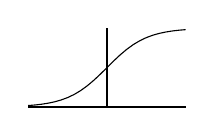
\begin{tikzpicture}[baseline={(0,0.2)}]
         \draw (-1,0) -- (1,0);
         \draw (0,0) -- (0,1);
         \draw plot[domain=-1:1,variable=\x] ({\x},{1/(1+exp(-4*\x))});
        \end{tikzpicture}\\
        \\
        tanh & $\sigma(x)=\frac{e^x-e^{-x}}{e^z+e^{-z}} $ & $\sigma'(x)=1-\sigma^2$   
        &  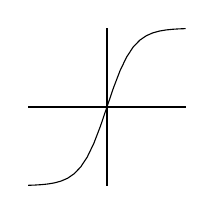
\begin{tikzpicture}[baseline={(0,0)}]
         \draw (-1,0) -- (1,0);
         \draw (0,-1) -- (0,1);
         \draw plot[domain=-1:1,variable=\x] ({\x},{tanh(3*\x)});
        \end{tikzpicture} \\
        ReLU & $\sigma(x) =\begin{cases}
        0 & ~\text{if}~ x<0 \\ 
        x & ~\text{if}~x \geq 0.
        \end{cases}$ & $\sigma'(x)=\begin{cases}
        0 & ~\text{if}~ x<0 \\ 
        1 & ~\text{if}~x > 0.
        \end{cases} $ & 
        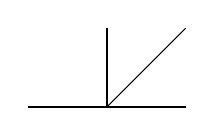
\begin{tikzpicture}[baseline={(0,0.5)}]
         \draw (-1,0) -- (1,0);
         \draw (0,0) -- (0,1);
         \draw plot[domain=-1:1,variable=\x] ({\x},{ifthenelse(\x<0,0,\x)});
        \end{tikzpicture}\\                      
    \end{tabular}
    \caption{Non-linear activation functions.}
    \label{tab:activationfct}
    \end{table}

\end{comment}

\section{Activation Functions}
There are many common activation functions with various strengths used in modern neural networks. We shall briefly mention a few ones
for completeness.

\subsection{Sigmoid and Tanh}
The sigmoid activation function is given by 
\begin{equation}\label{eq:sigmoid}
    \sigma(x) = \frac{1}{1 + \exp(-x)}.
\end{equation}
It was a very common choice in neural networks early, likely due to its simple derivative. It has a significant drawback, however.
Looking at eq.~\eqref{eq:sigmoid}, we can easily deduce that $\sigma(\pm \infty) = 0$, and since its derivative is of the form $\sigma'(x) = \sigma(1-\sigma)$,
the gradient computed during backpropagation vanishes if the input to the activation function as $\abs{x} \to \infty$. This significantly
hampers the progress during optimization. A popular alternative to the sigmoid function is $\tanh(x)$. This function is very similar to sigmoid in the sense that its derivative vanishes
for inputs of large magnitude and so may suffer from the same issues as sigmoid does.


\subsection{ReLU}
To overcome the vanishing gradient problem, an activation function called the Rectifying Linear Unit (ReLU) became widely adopted, which is given by
\begin{equation}
    \sigma(x) = x^+ = \max(0, x).
\end{equation}
% The activation was found to perform well in deep learning back in 2011 \cite{relu} and has become widely adopted.


\subsection{Swish}
Recently, an activation function to replace ReLU was proposed in \cite{swish} known as \textit{swish} or SiLU which was shown to outperform ReLU in deep neural networks on
a number of challengig datasets. The activation function is given by
\begin{equation}
    \sigma(x) = x\cdot \text{sigmoid}(x).
\end{equation}



\section{Bayesian learning of Neural Networks using Monte Carlo Samplers}
So far, we have discussed neural networks as a model class whilst ignoring the issue of what it really means to do Bayesian learning of neural networks, 
in other words, what it means to \textit{train} BNNs. We have intentionally left it somewhat ambigious what this really means because as it turns out, its meaning can be quite different depending on how Bayesian inference is performed. In this section we will clarify precisely what it means to train BNN using MCMC samplers such as HMC and NUTS. We shall then discuss practical aspects of the training which we shall put to practice in chapter \ref{chap:numerical_experiments}.

\subsection{What \textit{is} Bayesian learning of Neural Networks?}
The way Bayesian learning of neural networks manifest itself depends on the way in which we do Bayesian inference of the probabilistic model. 
We are concerned with inference of model parameters from the posterior using MCMC methods and will therefore obtain samples where each such sample
consist of the weights of an entire neural network. More precisely, if we gather $N$ samples with a chosen sampler, we will obtain $N$ entire neural networks
all sampled from the posterior to explain the observed data. Thus, what we mean by a \textit{trained} BNN in this sense is that we have
sampled a set of neural networks that collectively represent the BNN. 

As we discussed at the end of chapter \ref{chap:bayesian_ml}, 
we are mainly interested in the predictive distribution $p(y|x, W, b)$ of an output $y$ given an input $x$. We can approximate this distribution by constructing an empirical distribution by feeding $x$ through all $N$ sampled neural networks to obtain $N$ predicted targets $\hat{y}$ using eq.~\eqref{eq:predictive_dist_approx}.
The second quantity of interest is expectations of target functions dependent on the model parameters. 
We can approximate any such expectation with an MCMC estimator as in eq.~\eqref{eq:mcmc_estimator} using all $N$ networks to evaluate the target function.


\subsection{The Potential Energy Function of Neural Networks}

We now turn to the Bayesian formulation of the neural network model for use with the samplers used in this thesis. Assume that we have picked an architecture for a neural network and wish to train it in the Bayesian sense.
For both HMC and NUTS, we need only specify a potential energy function for our model. The samplers
take care of the rest. Assume we are dealing with a dataset $D = \{(x^{(i)}, y^{(i)})\}_{i=1}^N$ where all $N$ points are independent and identically distributed.
Equation~\eqref{eq:potential_energy_bayesian} instructs us to specify a prior for the weights of the network, and a likelihood function that depends on the target and the model output, in order
to fully specify the potential energy function.
Common practice is to choose priors that are either Gaussian or Laplacian. We will operate with Gaussian priors, i.e.
\begin{equation}\label{eq:model_priors}
  P(W^\ell) \propto \exp\left(-\frac{\lambda_W}{2}\norm{W^\ell}_2^2\right) \qq{and} \qquad P(b^\ell) \propto \exp\left(-\frac{\lambda_b}{2}\norm{b^\ell}_2^2\right).
\end{equation}
We will not worry too much about the choice of priors as the term in the potential energy function that corresponds to the likelihood will be much larger in practice. The Gaussian priors serve roughly the same purpose as $L^2$-regularization does in classical ML.

The likelihood for regression from eq.~\eqref{eq:likelihood_fn} formulated in terms of a neural network $\hat{f}(x^{(i)};W, b)$ is
\begin{equation}
  p(D|W, b) = \exp \left(-\frac{1}{2\sigma^2}\sum_{i=1}^N\norm{y^{(i)} - \hat{f}(x^{(i)};W, b)}_2^2\right).
\end{equation} 
This is not the only valid choice for a likelihood function but it is the common choice since it can be identified with the Euclidean $L^2$-norm and
itself ``neat'' mathematical properties.

Combining the priors and the likelihood with eq.~\eqref{eq:loss_function_of_posterior} yields the potential energy function
\begin{equation}\label{eq:special_potential_energy}
  \mathcal{L} = \frac{1}{2\sigma^2}\sum_{i=1}^N \norm{y^{(i)} - f(x^{(i)}; W, b)}_2^2 + \frac{\lambda_W}{2} \sum_{\ell=1}^L \norm{W^\ell}_2^2 + \frac{\lambda_b}{2}\sum_{\ell=1}^L \norm{b^\ell}_2^2,  
\end{equation}
up to a constant. As we discussed in chapter \ref{chap:hmc}, the potential energy function also happens to be the typical loss function with $L^2$-regularization used in the classical ML which is why we denote it as $\mathcal{L}$. At this point, we have set up all the machinery we need to train BNNs. Our next topic of discourse is the practice of doing so.

\subsection{Practical Training of Bayesian Neural Networks}

Training BNNs in practice requires us to specify a fairly large number of hyperparameters to obtain a set of models. These are 
\begin{enumerate}
  \item \textbf{Neural network architecture}. We need to specify its number of layers, number of nodes and activation function per layer. 
  Once the BNN is trained, we store this information along with the model for future usage. The stored weights themselves will encode how many layers and nodes the model has but the activation functions must be stored in addition.
  \item \textbf{Number of results}. We must specify how many neural networks we want to sample and store. Because the weights must be stored in its entirety, we are forced to worry about the amount of disk space that is required to do so. For a fixed allocated disk space, we can obviously store a larger set of samples if the model is simple. As complexity increases, the number of samples we can store will necessarily decrease.
  \item \textbf{Number of burn-in steps}. We must decide how long we want to run the MCMC chain before we start storing results. If amount of disk space was no obstacle, this step would be considered entirely optional as we could simply store every single sample and make a thorough analysis of the chain's quality to determine when proper mixing is obtained. In practice, with TensorFlow's framework, we can make a predetermined set of burn-in steps to avoid unnecessary RAM usage.
  \item \textbf{Amount of thinning}. Since successive samples most likely will be correlated, we can specify how many samples we simply skip once we start gathering samples, i.e. after the burn-in period. Again, we could ignore this and do this manually with the chain but doing so becomes a question of amount of available VRAM, RAM and disk space. 
  \item \textbf{Hyperparameters specific to the samplers}. The samplers themselves carry their own hyperparameters. In the case of HMC, we must specify a fixed number of Leapfrog steps $L$. If we use the NUTS sampler, we must specify the maximum tree depth. Moreover, we must determine how much of the computing resources we allocate to adapting the step size used in the Leapfrog integrator.
  \item \textbf{Amount of pretraining}. An attempt to accelerate convergence of the MCMC chain can be achieved by pretraining the neural network using minimization methods with the backpropagation algorithm to bring the weights closer to a minima of the potential energy function (i.e. the loss function used in classical ML). Then the point estimate obtained at the end of the training is used as a starting point for the MCMC chain.
\end{enumerate}

\subsection{Training Algorithm of Bayesian Neural Networks}
In this section we shall turn our attention to an actual training algorithm for BNNs. Assume we pick a sampler $S$ that represents either HMC or NUTS and a specified permuation of the hyperparameters discussed in the last section. In practice we can summarize a training algorithm as follows.
\begin{enumerate}
  \item Initialize the weights of the model from the specified priors, i.e.
  \begin{equation}
    W^\ell \sim p(W^\ell) \qq{and} b^\ell \sim p(b^\ell) \qq{for} \ell=1,\ldots, L.
  \end{equation}
  \item Minimize the potential energy function $\mathcal{L}$ with respect to the weights of the model using an optimizer of your choice to obtain a point estimate for use as the initial state of the Markov chain.
  \item Initialize the Markov chain for a finite set of burn-in steps to achieve mixing using $S$. A proportion of the initial burn-in steps are used for step size adaptation, while the remaining are used for mixing.
  \item Gather samples by applying $S$ repeatedly, replacing the current weights of the model by the ones returned by $S$.  
\end{enumerate}


\begin{comment}
  
With the ingredients discussed hitherto, it is time to consider practical training of BNNs.
We can divide this process in two parts. First, we must choose the architecture of the model, which is tantamount to picking model class. This decision is similar in nature to the training of regular neural networks to obtain point estimates. Second, we must consider the sampling process of the model. There are several considerations to make here such as disk space, length of mixing, amount of thinning and so on.

\subsection{Sampling of Bayesian Neural Networks}
We may divide this procedure into several subcategories:
\begin{enumerate}
  \item Choosing sampler $S$.
  \item Amount of mixing. We must choose the number of burn-in steps to run the sampling process before we actually start gathering sampled NNs.
  \item Amount of thinning. Number of samples to skip per stored sample. 
  \item Number of NNs to sample. Since the way we do Bayesian learning of NNs here actually require us a set of full NNs and store them to disk, we must decide how many samples we want to gather.
\end{enumerate}


\begin{enumerate}
  \item Initialize the weights of the network sampled from the priors. 
  \item An \textit{optional step}: train the network using a minimization algorithm with $\mathcal{L}$ as loss to reach an initial network state in the high probability \textit{density} region of the posterior.
  This is done to reduce the number of burn-in steps needed for the the Markov chain to reach the stationary distribution. However, for sufficiently high-dimensional parameter spaces this 
  may lead to adverse effects since the typical set may not be close to any mode of the posterior.
  \item Perform a finite number of burn-in steps to facilitate mixing by application of $S$ repeatedly.
  \item Sample a set of neural network parameters from the posterior distribution by use of $S$ repeatedly.
\end{enumerate}

\end{comment}

% \chapter{Bayesian learning of Neural Networks with Variational Inference}
% Sampling directly from the neural network's posterior using Hamiltonian Monte Carlo yields an empirical distribution
that accurately reflects the true posterior of the model. This makes the method the useful for applications that
demands accuracy.
The method comes with some undesirable limitations, however. 
It is inherently a \textit{batch} algorithm that needs to revisit the whole dataset for each sample new sample it produces,
limiting the size of the dataset one can apply the method to. Moreover, once the training process is completed, 
the obtained empirical distribution of model parameters $\theta$ must be stored in its entirety which imposes
a constraint on the number of samples one can use per model, as well as the size of the neural network itself. 
Large neural networks require a large number of parameters, which provides yet another limit on the number of samples
that can be stored for the bayesian neural network. 

In this chapter, we will survey an approximate method to bayesian learning with neural networks that
uses \textit{variational inference}. We'll first cover the general theory of variational inference,
before we discuss how it applies to neural network models. 

\section{Variational Inference}
Variational inference replaces the sampling from the exact posterior with sampling from an approximation to the posterior distribution,
called the \textit{variational distribution}, denoted $q_\phi(\theta)$, where $\theta$ is the model parameters (i.e the weights of the neural network) and $\phi$ represents the variational parameters.

%\input{Sections/QFT/Axiomatic}
%\input{Sections/QFT/Pertubationtheory}
%\input{Sections/QFT/StandardModel}
%%%%%%%%%%%%%%%%%%%%%%%%%%%%%%%%%%%%%%%%%%%%%%%%%%%%%%%%%%%
%\input{Sections/QFT/MathematicalFormulationGaugeTheories}
%\input{Sections/QFT/WilsonGeometry}

%%%%%%%%%%%%% Wilson Line Properties %%%%%%%%%%%%%%%%%%%%%%%%
%\chapter{Wilson Line Properties}
%\input{Sections/WilsonLineProperties/CuspAnomalous}

%\chapter{Supersymmetry}
%\input{Sections/SUSY/Supersymmetry}

%%%%%%%%%%%%% QCD %%%%%%%%%%%%%%%%%%%%%%%%
% \chapter{Perturbative Quantum Chromodynamics}\label{Chap:pQCD}
% \input{Sections/QCD/LagrangianQCD}
% \input{Sections/QCD/DIS}
% \input{Sections/QCD/DrellYan}



%%%%%%%%%%%%% Conclusion %%%%%%%%%%%%%%%%%%%%%%%%%%
\chapter*{Conclusion}\label{chap:conclusion}
% \newpage
% \chapter*{Conclusion}
% \addcontentsline{toc}{chapter}{Conclusion}
The main objective of this thesis has been to investigate Bayesian neural networks sampled from the exact posterior as a substitute for direct calculations of next-to-leading order cross sections in quantum field theory. We argued for the necessity of bypassing the computationally expensive direct calculations with Bayesian regression because of the need for an estimate of the uncertainty of the predicted cross sections. This was due to the role the uncertainties play in the statistical exclusion of regions in parameter spaces of possible Beyond the Standard Model theories. The neural network model was chosen for its universal function approximation property. We provided an overview of Bayesian machine learning and its relation to classical machine learning with a focus on regression tasks. We sought to use Markov chain Monte Carlo methods to sample from the exact posterior of neural networks and thus delved into the theory behind these methods for continuous sample spaces, building our way through the Metropolis-Hastings methods all the way up to the advanced class of samplers used in this thesis, namely Hamiltonian Monte Carlo. We discussed the shortcomings of Hamiltonian Monte Carlo with a fixed trajectory length and its need for tedious hand-tuning via preliminary diagnostic tests. This motivated the exploration of adaptive Hamiltonian Monte Carlo techniques to adapt the trajectory length with the No-U-Turn sampler for the number of Leapfrog steps and a dual-averaging scheme for the step size used in the Leapfrog integration component. 

Through numerical experiments, we demonstrated that trained BNNs can significantly reduce the time spent computing cross sections. We found that the time spent on such computations were roughly evenly divided between loading the models in from memory and performing the actual forward pass in the neural networks to compute the predictive distribution, its sample mean and sample variance. Moreover, we found that the training employed on GPUs with XLA compilation can result in a significant reduction in training time compared to training on CPUs.
We investigated the empirical posterior distribution of the sampled weights and found them to be multi-modal, consistent with claims in the literature, sowing doubt of the reliability of Bayesian inference using surrogate models. We explored how various hyperparameters used during training of BNNs affect their predictive performance. We found evidence suggesting that a moderate amount of warm-up steps and pretraining positively impacts the performance of the trained models but that an excessive amount exacerbated it. With the vast set of different configurations one can use with BNNs though, these results may not be generalizable to different forms of architectures than the ones we have used and more extensive investigations can be carried out. Some of the configurations we explored were found to produce reliable uncertainty estimates and performed well in the space of targets it was trained for. Finally, we explored the predictive distributions of a trained BNN model and showcased an example of a good predictive distribution and a predictive distribution which missed the mark entirely. We showed that the BNN model underperformed relative to a Normal distribution where less than 96 \% of the targets resided within $\pm 2\sigma$ of the sample mean of the distributions. 

Although we have progressed our understanding of the training of BNNs by drawing samples from the exact posterior with MCMC samplers like HMC and NUTS, there are several question which we have not answered. We propose the following problems to be addressed in the future.
\begin{enumerate}
    \item \textbf{The Convergence Properties of the Markov Chain}. In chapter \ref{chap:mcmc}, we noted that the standard metric to estimate that a Markov chain has converged to its stationary distribution were by use of the scale reduction factor $\hat{R}$. Such convergence statistics is not measured or reported in this thesis. Computing $\hat{R}$ for neural network posteriors is complicated by the non-identifiability of neural networks. Several different neural networks sampled from the different regions of sample space may produce the same predictions, which makes assessing the convergence by studying the elements of the Markov chain itself challenging. Instead we propose the use of $\hat{R}$ computed on the predictions by using the samples in the Markov chain. This analysis has been performed in \cite{google_bnn_posteriors} where they study the resulting Markov chain in function space. For a specific input $x$, one can run several independent chains that all compute their own predictive distribution. The $\hat{R}$ metric can then be calculated from the resulting set of distributions to identify potential non-convergence.
    \item \textbf{Training of BNNs on Larger Datasets}. In this thesis, we have focused on a fairly small dataset of $\sim 15000$ datapoints. At no point have we investigated the added computational expense from computing the potential energy function and its gradient in HMC and NUTS as a function of the number of datapoints it needs to be evaluated for. If NLO cross section estimation is to be used with BNNs on larger datasets, the effect it has on the hyperparameters used during training is likely necessary to be reinvestigated. The analysis performed in this thesis should at least give information on what hyperparameters that are worth exploring. Training time will likely be much longer but the predictive performance of the trained BNN may become more robust.
    \item \textbf{Sampling Larger Models}. Our analysis has been dealing with a fairly small number of sampled neural networks per model. In each case, we have drawn 1000 neural networks which collectively represented the full BNN model. The number of parameters the models had, spanned from a few hundred to the order of a hundred thousand. A thousand samples drawn from the posterior is a pretty low number owed to the computational expense needed to generate them. For the most complex models trained, the training time could exceed 24 hours on a GPU. Thus drawing more samples by running longer Markov chains can be exceedingly expensive. The potential upside is that the MCMC estimators and the predictive distributions will likely produce better results if more samples are drawn. An important consideration to reduce the training time is to increase the complexity of neural networks by adding many small layers and create deep networks as opposed to shallow networks with many nodes per layer. The reason for this is that applying shallow ``wide'' networks to a large dataset simultaneously during training may create temporary objects which are too large to fit into cache and registers which results in additional time spent transferring strips of memory, in which case the GPU may sit idle during large portions of the training.
    \item \textbf{The Effect of Thinning}. We have operated with a fixed number of samples skipped between each drawn network. This means that we have performed no analysis of the correlation between successively drawn samples but instead worked with a heuristic that appeared to produce good results. Investigating the \textit{lag}-$l$ autocorrelation of successive neural network samples can give valuable information from a practical perspective. Although drawing more samples may be beneficial for the calculation of MCMC estimators, it is not so if the samples are heavily correlated. Both samplers used in this thesis generate successive samples with low correlation in simple cases studied in the literature \cite{nuts,neal2011} but with the complexity of the BNN posterior, this may require a larger amount of thinning. Performing preliminary runs to estimate how correlated successive samples are will help reduce the necessary amount of samples needed to be drawn to obtain good statistics from the MCMC estimators. It will also help the practitioner to minimize the amount of thinning and avoid wasting computational resources.
    \item \textbf{The Effect of the Multi-modality of the Posterior on the Predictive Distributions}. Although we demonstrated the multi-modality of the posterior distribution of BNNs, we did not investigate its effect on the predictive distribution. After all, it is the predictive distribution we really care about in practice. Due to how computationally expensive it is to sample from the exact posterior, a thorough comparison of sampling from the exact posterior should be compared and contrasted with the use of surrogate distributions for the BNNs parameters with respect to the quality of the predictive distributions they produce.
    \item \textbf{Other Potential Energy Functions}. In our investigation we have used a Gaussian prior for each neural network parameter and the same likelihood function for each model. It is possible that modifying the potential energy function, either by choosing different priors or modifying the likelihood function, that the training process can be improved. It has been suggested that the effect of the chosen priors may yield a measurable impact on the predictive distribution although it may not be particularly noticable from studing the posterior distribution of weights \cite{google_bnn_posteriors}.
    \item \textbf{Deep Ensembles}. Deep ensembles has been shown to yield a better fidelity of the Bayesian predictive distribution on par with the ones produced by HMC, outperforming the surrogate distributions typically employed in the literature \cite{google_bnn_posteriors}. And this can potentially be achieved at a significant reduction of the computational cost of sampling from the true posterior using HMC or NUTS. 
    \item \textbf{Multi-GPU Training with HMC}. In this thesis, within the framework we used, we were confined to run the sampling on a single GPU device. Investigating the possibility of running multiple independent Markov chains on several GPUs simultaneously in an asynchronous fashion can potentially speed up the training of BNNs with HMC significantly by allowing for many long chains to sample independently of each other. The quality of the sampled chains from the posterior is likely to improve by generating more than a single chain. One possible framework to adopt for this is Jax \cite{jax}, a machine learning research library developed and used in-house by the Deep Mind research team at Google Research. It allows for automatic mapping of a Python function to several physical devices (such as multiple GPUs), just-in-time compilation for GPU devices which when run on NVIDIA GPUs support XLA compilation. Moreover, it provides its own framework for automatic differentiation. Thus it may be a viable platform to develop more research oriented machine learning models than the more strict frameworks provided by TensorFlow and its extensions. Due to the complex control flow introduced by the NUTS sampler, it is not as well suited for multi-GPU sampling but other adaptive schemes such as ChEES-HMC was recently proposed to adaptively set the trajectory length without the same limitation \cite{chees-hmc}.
    \item \textbf{Approximate the Prior From the Empirical Distribution for Online Training}. A major drawback to drawing samples from the exact distribution is that we in practice must discard old models when new data becomes available. This is unfortunate as we obviously know \textit{something} about the weights inferred from the dataset prior to the arrival of the hypothetical new data. We are closely guarding a set of them which we have drawn, informed by the ``old'' data. In order to increase the viability of sampling from the exact posterior, investigating ways to obtain approximate unnormalized densities that approximate the empirical distributions can be fruitful for the following reason. The potential energy function used in HMC and NUTS \textit{requires} the ability to evaluate a log prior given an arbitrary input of weights. Thus inferring a function that approximates the empirical distribution will yield an \textit{informed} prior that can be evaluated to draw new samples given new data. This can greatly increase the viability of the methods as old samples can inform the generation of new ones. 
\end{enumerate}
\backmatter{}
%%%%%%%%%%%%% Appendix %%%%%%%%%%%%%%%%%%%%%%%%

\begin{appendices}
\numberwithin{equation}{section}

\appendix
\chapter{Appendix A}
\renewcommand{\thechapter}{A}
\renewcommand{\theequation}{\thechapter.\arabic{equation}}
\section{Appendix 1 title }\label{sec:appendix_1_label}
Some appendix stuff.



% \appendix
% \renewcommand{\thechapter}{B}
% \chapter{Appendix B}
% \input{Sections/Appendix/Appendix2}
%
% \appendix
% \renewcommand{\thechapter}{C}
% \chapter{Appendix C}
% \renewcommand{\theequation}{\thechapter.\arabic{equation}}
% \input{Sections/Appendix/Appendix3}
%
% \appendix
% \renewcommand{\thechapter}{D}
% \chapter{Appendix D}
% \renewcommand{\theequation}{\thechapter.\arabic{equation}}
% \input{Sections/Appendix/Appendix4}


\end{appendices}




\bibliography{bibliography.bib}

\end{document}
